% asset_id: FAS2GeometricDistributionTikZ-002 optional
\documentclass[tikz,border=8pt]{standalone}
\usepackage{amsmath}
\usetikzlibrary{decorations.pathreplacing}
\begin{document}
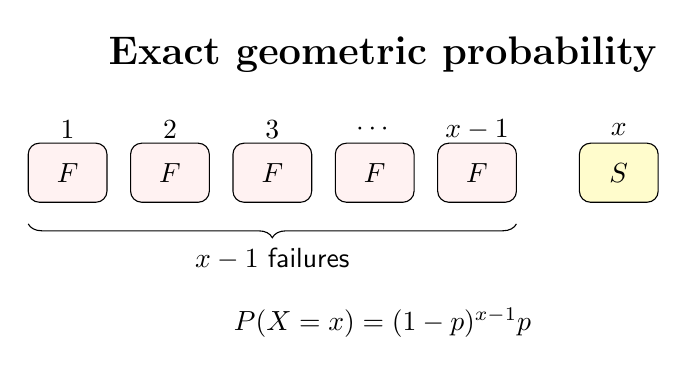
\begin{tikzpicture}[font=\sffamily]
\node[font=\bfseries\Large] at (5,3) {Exact geometric probability};
\foreach \i/\lab in {0/1,1/2,2/3,3/\cdots,4/x-1}{\node[draw,rounded corners,fill=red!5,minimum width=1cm,minimum height=.75cm] at (1+\i*1.3,1.5) {$F$};\node at (1+\i*1.3,2.05) {$\lab$};}
\node[draw,rounded corners,fill=yellow!20,minimum width=1cm,minimum height=.75cm] at (8.0,1.5) {$S$};\node at (8,2.05) {$x$};
\draw[decorate,decoration={brace,mirror,amplitude=5pt}] (.5,.85)--(6.7,.85) node[midway,yshift=-.45cm] {$x-1$ failures};
\node at (5,-.4) {$P(X=x)=(1-p)^{x-1}p$};
\end{tikzpicture}\end{document}
